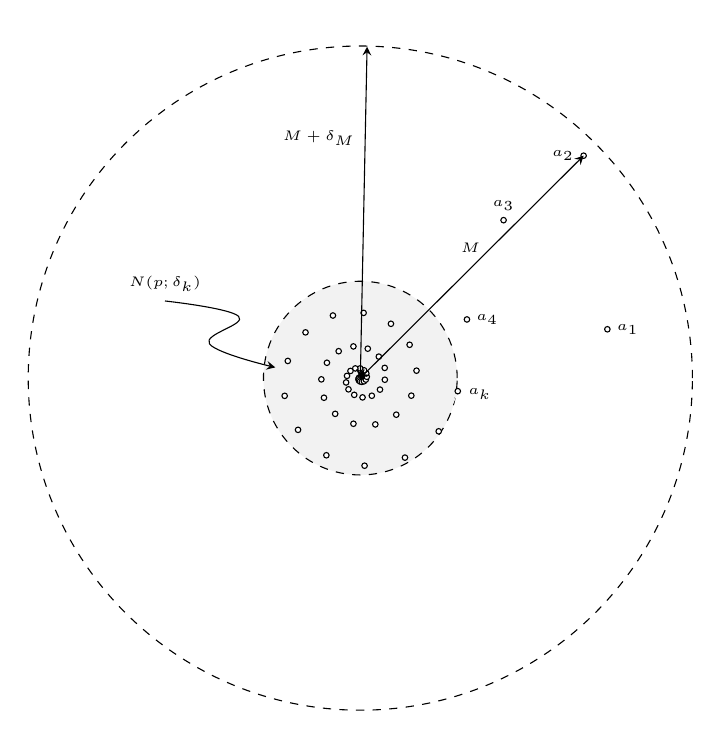
\begin{tikzpicture}
   \coordinate (O) at (0,0) {} {} {};
   \draw[dashed,fill=gray!10]  (O) circle (35pt);
\draw [gray!10,domain=0:25,variable=\t,smooth,samples=55]    plot[mark=*,mark size=1pt,,mark options={black,fill=white}] ({\t r}: {0.002*\t*\t});
   \coordinate (a3) at (1.3542,0.7447) {};
      \coordinate (a2) at (1.8193,2.0056) {} {} {} {} {};
  \coordinate (a1) at (2.836,2.8246) {} {};
   \coordinate (a0) at (3.1376,0.62) {} {} {};
\draw [white] plot[white,mark=*,mark size=1pt,,mark options={black,fill=white},smooth, tension=.7] coordinates {(a0) (a1) (a2) (a3)};

      \coordinate (O) at (0,0) {} {} {};
   \draw[dashed]  (O) circle (120pt);
   \node[right] at (a0) {\tiny$a_1$};
   \node[left]  at (a1) {\tiny$a_2$};
   \node[above]  at (a2) {\tiny$a_3$};
   \node[right]  at (a3) {\tiny$a_4$};
   \coordinate (ak) at (1.25,-0.2) {} {} {};
     \node[right]  at (ak) {\tiny$a_k$};
\node (v1) at (0.0885,4.3332) {};
\draw[<->,>=stealth]  (O)--(a1);
\node at (1.4005,1.6608) {\tiny$M$};
\draw[<->,>=stealth]  (O)--(v1);
\node[left] at (0.0577,3.0487) {\tiny$M+\delta_M$};
\draw[->,>=stealth]  plot[smooth, tension=.7] coordinates {(-2.4807,0.9793) (-1.5451,0.784) (-1.9152,0.4344) (-1.08,0.136)};
\node[above] at (-2.4807,0.9793) {\tiny$N(p;\delta_k)$};
\end{tikzpicture}